\chapter{Sensores RGB-D}
El área de visión en computación es un área de investigación que está constantemente en desarrollo y la cual tiene cada vez más aplicaciones en problemas del mundo real. Durante los últimos años y con el poder de cómputo de los nuevos procesadores se ha posibilitado el desarrollo de nuevos y mejores algoritmos utilizando más información del entorno, manteniendo tiempos de ejecución razonables para aplicaciones de tiempo real.

Dentro de estos avances logrados en el área, los sensores RGB-D otorgan una novedosa forma de obtener datos visuales del ambiente. Estos sensores están conformados típicamente por una cámara tipo web común RGB que captura el mundo en dos dimensiones (2D), es decir, las texturas o colores del mundo real y por otra parte tienen una cámara de profundidad que provee información de la distancia de los distintos objetos de la escena a la cámara.

La cámara o sensor de profundidad consta de dos elementos: un proyector infrarrojo y una cámara infrarroja. Para poder medir la profundidad de todo lo presente en la escena el proyector imprime con luz infrarroja un patrón conocido. Esta luz es invisible al ojo humano y a las cámaras RGB convencionales. Sin embargo, si se puede ver con una cámara infrarroja. La cámara infrarroja entonces, se utiliza para obtener el patrón dibujado en la escena. Conociendo el patrón original proyectado, el patrón obtenido con la cámara y la distancia entre la cámara y el proyector se pueden aplicar algoritmos de luz estructurada para obtener la profundidad de la escena.

Existen varias implementaciones de cámaras que otorgan esta información y cada una tiene sus propias características en cuanto a calidad de la imagen RGB, frecuencia de cuadros, rango de profundidad, etc. La más conocida de estas cámaras es la llamada ``Kinect'' de Microsoft. Esta cámara posee una resolución default en RGB de unos 640x480 pixeles de 8 bits cada uno, a unos 30 cuadros por segundo. La misma puede otorgar imágenes de hasta 1280x1024 pixeles pero a una frecuencia de cuadros menor. En el caso del video en profundidad, el sensor provee una resolución de imagen de unos 640x480 pixeles y cada uno de ellos tiene una resolución de 11 bits, lo que da una sensibilidad de 2048 niveles. La frecuencia de cuadros que otorga el sensor de profundidad es de unos 30 cuadros por segundo. El rango práctico de distancias que ofrece la cámara está entre 1.2 y 3.5 m, aunque puede dar un rango extendido de unos 0.7 a 6 m.

Una de las características de los sensores de profundidad de este tipo es que al utilizar luz infrarroja no necesitan luz para sensar y obtener información. De manera contraria a una cámara RGB, este sensor se ve perjudicado por la luz solar ya que el sol emite luz infrarroja que interfiere con el patrón dibujado por el proyector, haciendo que los datos sensados no sean correctos. Además el método se ve perjudicado cuando existen en la escena objetos como vidrios, espejos y superficies brillantes ya que los haces de luz son reflejados y por lo tanto se modifica el patrón proyectado por el sensor.


\section{Lluvia de ideas}
Sensores RGB-D (lluvia de ideas)
- Explicar qué son:

- Ejemplos de imágenes y point clouds
- mediante los parámetros de calibración de las cámaras se pueden obtener los puntos 3D de la escena capturada junto con su información de color o textura asociada. Explicar un poco cómo.
- Ventajas de contar con info 3D. 
- Diferencia entre los mundos 2D y 3D. En una cámara 2D, el mundo es proyectado,  se pierde la información de profundidad de los tamaños, problema de la escala. Mientras que en el mundo 3D es el mundo como lo percibimos los seres humanos.
- Aplicaciones en entretenimiento y en la industria




\chapter{Sistema de seguimiento en video}

Un sistema de seguimiento en video se puede dividir en tres etapas bien definidas:
\begin{enumerate}
 \item Entrenamiento
 \item Detección
 \item Seguimiento cuadro a cuadro
\end{enumerate}

La etapa de entrenamiento consiste en obtener una representación del objeto al cuál se pretende seguir. Para llevarla a cabo se puede utilizar un patrón \textit{template} ya conocido o aprenderlo de imágenes capturadas del mismo objeto. Luego, este se utilizará en la detección para ubicar la representación del objeto dentro de una imagen cualquiera. Una vez conocido el \textit{template} no se requiere de una nueva ejecución del entrenamiento.

La segunda etapa, la de detección, radica en encontrar dentro de un cuadro del video al objeto en cuestión utilizando el método de detección deseado, valiéndose de la información obtenida en la etapa de entrenamiento. Esta etapa se ejecuta, con el propósito de encontrar en la imagen el objeto a seguir, al comienzo del sistema de seguimiento y cuando el seguimiento cuadro a cuadro falla. Dado que la etapa de detección suele ser la más costosa en términos de desempeño computacional es deseable que se ejecute la menor cantidad de veces posible.

Finalmente, la tercera etapa consiste en seguir cuadro a cuadro el objeto detectado en la etapa anterior. Es decir, teniendo la ubicación del objeto en un cuadro de video se desea identificar la posición del mismo objeto en el siguiente \textit{frame}. Esta etapa es la más importante ya que es la que se ejecuta en cada frame del video. La eficiencia del método de seguimiento cuadro a cuadro es lo que determinará que todo el sistema de seguimiento se consiga realizar eficientemente. Si la técnica de seguimiento tiene una efectividad baja, es decir, no logra identificar la nueva posición del objeto en el siguiente cuadro, se debe volver a la etapa de detección degradando el desempeño de todo el sistema.

Tomando como base estas etapas, proponemos distintos métodos para cada una de ellas tanto para imágenes sólo RGB, como para \textit{depth} (profundidad) y la combinación RGB-D. La primera etapa del sistema puede ser prescindible si contamos con el modelo RGB-D del objeto a seguir y una cámara calibrada. Este es el caso de estudio de esta tesis, ya que, con el propósito de poder evaluar cuantitativamente el seguimiento de objetos en secuencias de imágenes RGB-D, utilizamos la base de datos con ground truth descripta en la sección \ref{base_rgbd}.

\section{Método propuesto RGB}\label{metodo_rgb}
En esta sección explicaremos como se implementó el sistema de seguimiento para secuencias de imágenes RGB basándonos en las etapas explicadas previamente.

\subsection{Entrenamiento}
La etapa de entrenamiento en este método consta de tomar de la base de datos cuatro templates del objeto que se desea seguir con sus respectivas máscaras. Cada uno de los templates corresponde a una pose distinta. Primero se elige de manera arbitraria una de las varias escenas por objeto que tiene la base de datos. Una vez elegida la escena se toman cuatro templates de manera que se cubran las distintas caras del objeto. Si se toma la primer imagen de la escena como la imagen con rotación 0 el resto de las imagenes se eligieron de manera tal que cada una difiera de la anterior en 90 grados. En la figura \ref{templates_objeto} se pueden ver los distintos templates tomados de esta manera para un objeto de la base de datos. Una vez almacenados estos templates y sus respectivas máscaras se pasa a la etapa de detección.

\begin{figure}
	\centering
	\begin{subfigure}[b]{0.25\textwidth}
		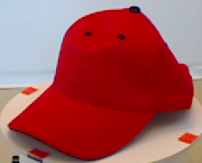
\includegraphics[width=\textwidth]{img/0_crop.png}
		\caption{Rotacion $0^{\circ}$}
	\end{subfigure}
	\quad
	\begin{subfigure}[b]{0.25\textwidth}
		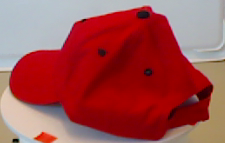
\includegraphics[width=\textwidth]{img/90_crop.png}
		\caption{Rotacion $90^{\circ}$}
	\end{subfigure}

	\begin{subfigure}[b]{0.25\textwidth}
		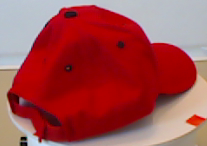
\includegraphics[width=\textwidth]{img/180_crop.png}
		\caption{Rotacion $180^{\circ}$}
	\end{subfigure}
	\quad
	\begin{subfigure}[b]{0.25\textwidth}
		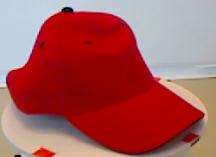
\includegraphics[width=\textwidth]{img/270_crop.png}
		\caption{Rotacion $270^{\circ}$}
	\end{subfigure}
	\caption{Templates de una gorra tomados de la base de datos}
	\label{templates_objeto}
\end{figure}

\subsection{Detección}
Dada la información provista por la base de datos, aprovechada durante el entrenamiento, resulta natural utilizar como método de detección el algoritmo de \textit{Template matching}. \comentarioM{Hay que explicarlo, ¿no?} La implementación utilizada es la que se encuentra presente en la librería \textit{OpenCV} para C++. Esta implementación recibe varios parámetros. El primero es el frame de la escena a donde se desea detectar el objeto. El segundo es el template con el que se va a buscar el objeto. El tercero es opcional y es una máscara para el template del objeto. En este caso como tenemos la máscara disponible este parámetro lo usamos. El último parámetro le indica al algoritmo de template matching que comparación usar para matchear el template a la imagen. Nosotros decidimos utilizar la diferencia cuadrática pixel por pixel normalizada, descripta por la siguiente fórmula:

\comentarioM{Insertar formula aqui.}% http://docs.opencv.org/modules/imgproc/doc/object_detection.html?highlight=matchtemplate#matchtemplate

Pero aplicar este método de manera directa no es suficiente. El problema principal es que la escena de donde se obtuvieron los templates y máscaras del objeto a buscar no es la misma escena que la que se utiliza para verificar el comportamiento del sistema. Esto significa que las poses del objeto tomadas en la etapa de entrenamiento pueden ser completamente distintas a las poses del objeto en la escena en donde se aplica el sistema de seguimiento. Además, la distancia de la cámara al objeto en la escena de búsqueda varía constantemente y difiere de la distancia entre ambos en la escena de donde se capturó el modelo del objeto. Por este motivo también va diferir la escala del objeto en cada escena.

Teniendo en cuenta estos problemas decidimos realizar varias corridas del algoritmo de \textit{template matching}. En primera medida en cada pasada se va modificando el par template-máscara utilizados como parámetros del mismo aprovechando los datos obtenidos en la etapa de entrenamiento. Con esto se ataca de mejor manera el problema de las distintas poses en las que puede estar el objeto en la escena. Además, para que la detección sea más robusta frente a cambios de tamaño del objeto que se desea encontrar se toma a cada uno de los templates con su respectiva máscara y se les aplican varios cambios de escala y se utilizaron estas muestras como entrada para el algoritmo de template matching. Una vez corrido el algoritmo para cada par template-máscara, se obtiene como resultado final la corrida que tenga menor diferencia cuadrática y que esté por debajo de un umbral predefinido. La información que se almacena como resultado son las coordenadas del cuadrante que contiene al objeto encontrado. Una vez almacenada esta información, el sistema pasa a la etapa de seguimiento.

\subsection{Seguimiento}\label{tracking_rgb}
Como se explicó al comienzo del capítulo, esta etapa consta de seguir al objeto detectado en la etapa anterior frame a frame. Para concretar este objetivo se necesita encontrar una manera de combinar la información obtenida durante las dos etapas anteriores. Existen muchas maneras de llevar a cabo esta tarea. La forma que elegimos para este trabajo fue utilizar un método de comparación por histogramas.

Cada imagen RGB consta de tres imagenes, una por cada canal. Para calcular el histograma de una imagen se toman los distintos valores (intensidad) de cada pixel y se cuenta la cantidad de veces que se repite cada uno de esos valores en la imagen. Las imágenes que utilizamos durante el transcurso de este trabajo son de 8 bits por pixel, por lo que cada pixel puede tomar un valor entre 0 y 255. Para que las comparaciones entre histogramas sean más robustas lo que se decidió fue trabajar con histogramas normalizados.


\begin{figure}
	\centering
	\begin{subfigure}[b]{0.25\textwidth}
		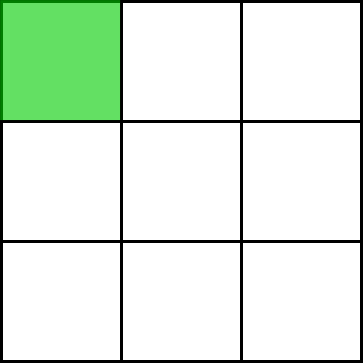
\includegraphics[width=\textwidth]{img/primercuadrante.png}
		\caption{Primer frame de búsqueda}
		\label{frames_solapados_1}
	\end{subfigure}
	\quad
	\begin{subfigure}[b]{0.25\textwidth}
		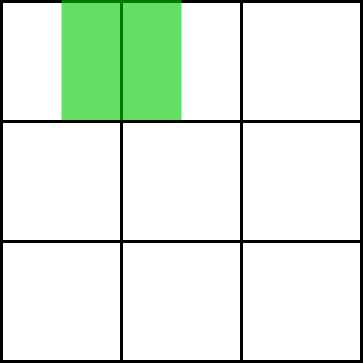
\includegraphics[width=\textwidth]{img/segundocuadrante.png}
		\caption{Segundo frame de búsqueda}
		\label{frames_solapados_2}
	\end{subfigure}
	\quad
	\begin{subfigure}[b]{0.25\textwidth}
		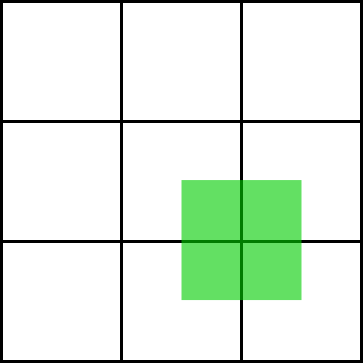
\includegraphics[width=\textwidth]{img/decimonovenocuadrante.png}
		\caption{$19^{\circ}$ frame de búsqueda}
		\label{frames_solapados_3}
	\end{subfigure}
	\caption{Se busca en cada cuadrante de la grilla y en los recuadros del mismo tamaño que cubren los bordes de la grilla principal}
	\label{frames_solapados}
\end{figure}


El algoritmo de tracking implementado se puede separar en dos partes. Por un lado tenemos el método de búsqueda y por el otro el algoritmo de comparación por histogramas. El método de búsqueda se utiliza para explorar un espacio predefinido en donde se asume estará el objeto en el siguiente frame. Este algoritmo toma un área de tamaño 9 veces mayor a la del cuadrante reportado por el algoritmo de detección respetando el centro del mismo. Luego divide esta área en cuadrantes los que serán utilizados por el algoritmo de comparación para definir si el objeto está o no allí. En la figura \ref{frames_solapados} se muestra una secuencia de búsqueda por cuadrantes. Para hacer más robusta la búsqueda frente a cambios de tamaño del objeto este mismo método de búsqueda por cuadrantes se realiza varias veces cambiando el tamaño del cuadrante.

La segunda parte del algoritmo de tracking consta en definir cuál de todos los cuadrantes explorados en la etapa de búsqueda es el que contiene el objeto que se está buscando o en caso de fallar en la búsqueda, indicar que el objeto no se encontró en el frame. En un principio en esta etapa se comparaba el histograma de cada uno de los cuadrantes explorados con el cuadrante del frame anterior reportado por el algoritmo de detección. Para esta comparación se tomaba de cada recuadro su histograma para los canales S y V del esquema de colores HSV y se los comparaba utilizando la implementación de comparación de histogramas presente en la librería OpenCV. El método de comparación utilizado se basaba en la diferencia de \textit{Bhattachayyra}. El resultado de estas comparaciones era aquel cuadrante cuya comparación arrojara el menor valor y que se encontrara por debajo de un umbral definido. Si ningún cuadrante arrojaba una comparación menor a este umbral el algoritmo indicaba que el objeto no se encontraba en ese frame.

El problema con esta aproximación era que al basarse únicamente en el recuadro encontrado en el frame anterior el objeto iba quedando de a poco fuera del recuadro resultante hasta que en un momento quedaba completamente fuera del mismo. Como la diferencia entre los cuadrantes resultantes de cada frame era baja, el algoritmo seguía reportando al objeto como encontrado aunque no fuera así. Para evitar este inconveniente se decidió además comparar el histograma de cada cuadrante de búsqueda con el histograma de uno de los templates del objeto obtenido en la etapa de entrenamiento. En este caso la comparación se realizó utilizando el esquema RGB, calculando el histograma para los tres canales. En las figuras \ref{frame_only_tracking} y \ref{frame_template_tracking} se pueden ver dos secuencias del algoritmo de seguimiento, una con comparación de histogramas unicamente entre frame y frame y otra que agrega además la comparación con el template del objeto respectivamente. El cuadrante de color verde es el reportado por el ground truth como la ubicación del objeto en la escena, en este caso, una taza. El cuadrante de color azul es el reportado por nuestro algoritmo. En la figura \ref{frame_only_tracking} podemos ver como frame a frame el cuadrante azul se va alejando de la taza hasta que en el frame 8 de este extracto de la escena el algoritmo indica que encontró a la taza en una zona que en realidad es parte de la notebook. En la figura \ref{frame_template_tracking} podemos ver en cambio que el área reportada por el algoritmo se mantiene más estable. En el frame 7 aparece un recuadro rojo. Eso significa que el algoritmo de seguimiento perdió el rastro del objeto y en ese frame hizo falta correr el algoritmo de detección. Luego, en los frames 8 y 9 el algoritmo no reporta haber seguido al objeto. Por este motivo es que se decidió utilizar la comparación de histogramas tanto con el frame anterior como con el template del objeto.

\comentarioM{¿Explico porque se eligió HSV y RGB en cada caso?}

\begin{figure}
	\centering
	\begin{subfigure}[b]{0.3\textwidth}
		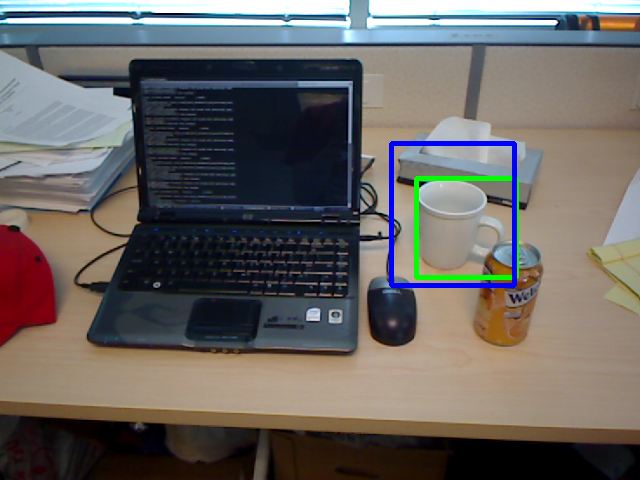
\includegraphics[width=\textwidth]{img/seguimiento_solo_frame/solo_frame-desk_1-coffee_mug_5-frame_26.png}
	\end{subfigure}
	\begin{subfigure}[b]{0.3\textwidth}
		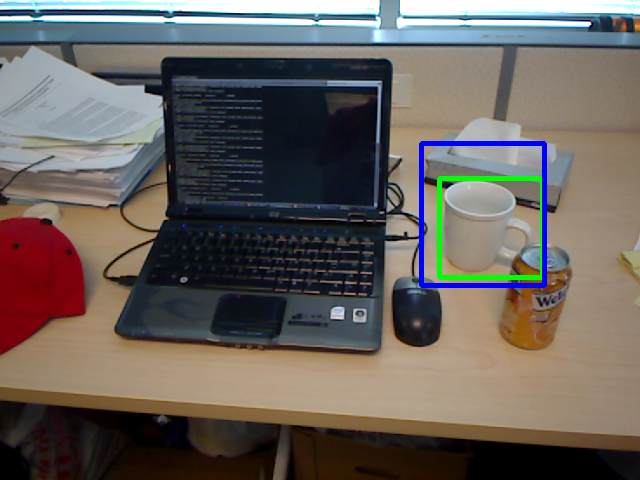
\includegraphics[width=\textwidth]{img/seguimiento_solo_frame/solo_frame-desk_1-coffee_mug_5-frame_27.png}
	\end{subfigure}
	\begin{subfigure}[b]{0.3\textwidth}
		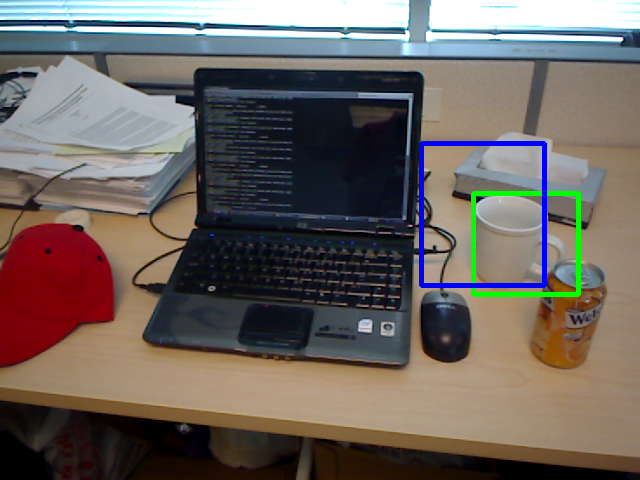
\includegraphics[width=\textwidth]{img/seguimiento_solo_frame/solo_frame-desk_1-coffee_mug_5-frame_28.png}
	\end{subfigure}


	\begin{subfigure}[b]{0.3\textwidth}
		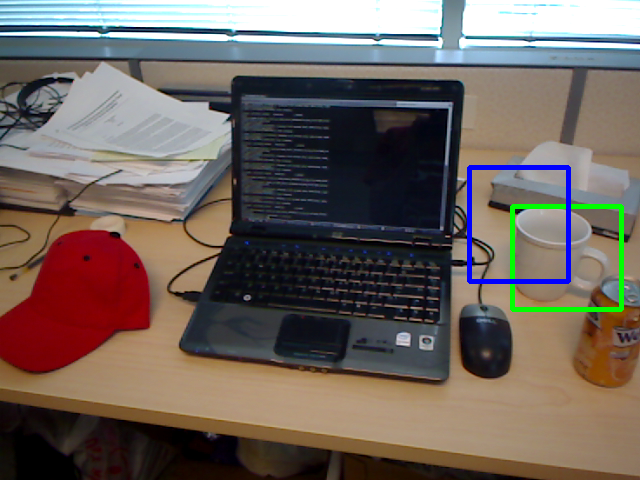
\includegraphics[width=\textwidth]{img/seguimiento_solo_frame/solo_frame-desk_1-coffee_mug_5-frame_29.png}
	\end{subfigure}
	\begin{subfigure}[b]{0.3\textwidth}
		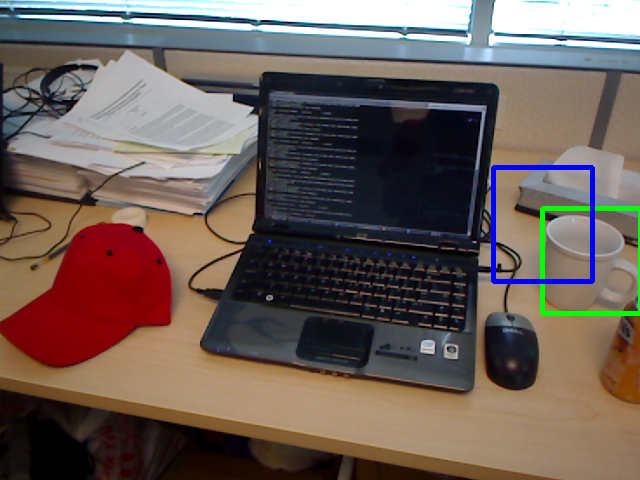
\includegraphics[width=\textwidth]{img/seguimiento_solo_frame/solo_frame-desk_1-coffee_mug_5-frame_30.png}
	\end{subfigure}
	\begin{subfigure}[b]{0.3\textwidth}
		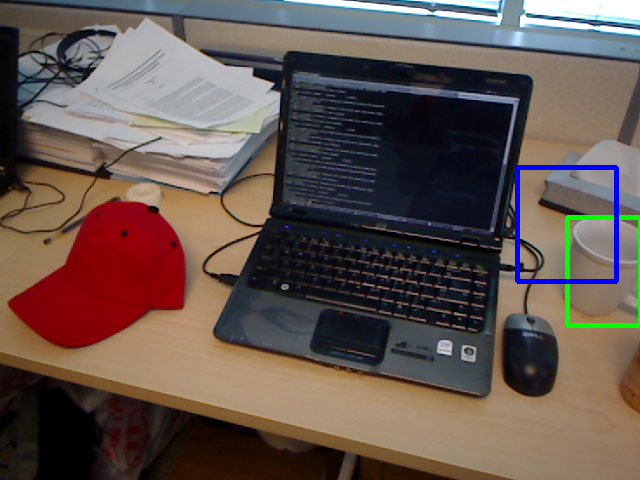
\includegraphics[width=\textwidth]{img/seguimiento_solo_frame/solo_frame-desk_1-coffee_mug_5-frame_31.png}
	\end{subfigure}

	\begin{subfigure}[b]{0.3\textwidth}
		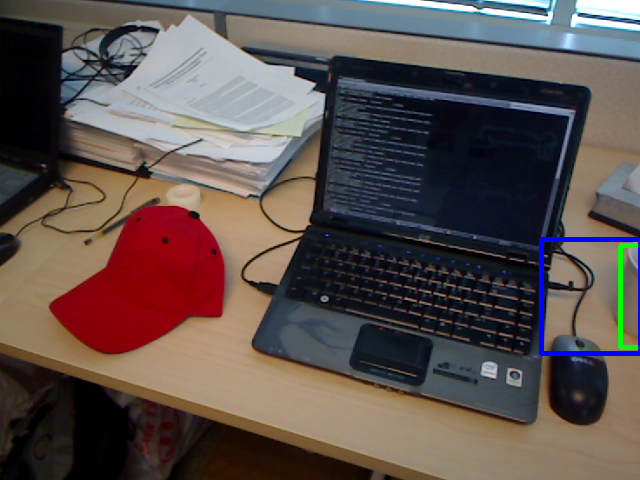
\includegraphics[width=\textwidth]{img/seguimiento_solo_frame/solo_frame-desk_1-coffee_mug_5-frame_32.png}
	\end{subfigure}
	\begin{subfigure}[b]{0.3\textwidth}
		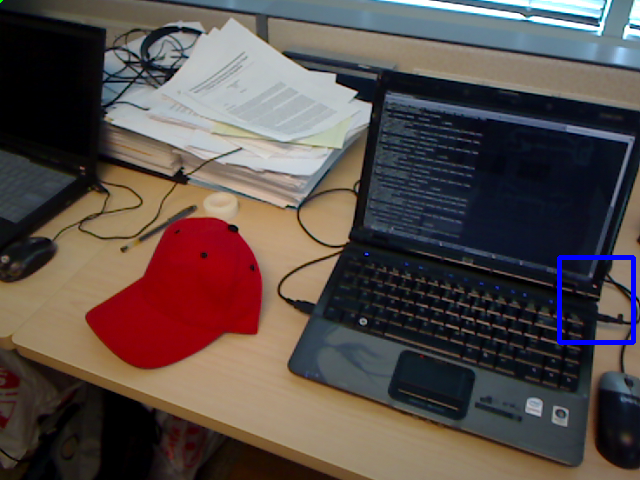
\includegraphics[width=\textwidth]{img/seguimiento_solo_frame/solo_frame-desk_1-coffee_mug_5-frame_33.png}
	\end{subfigure}
	\begin{subfigure}[b]{0.3\textwidth}
		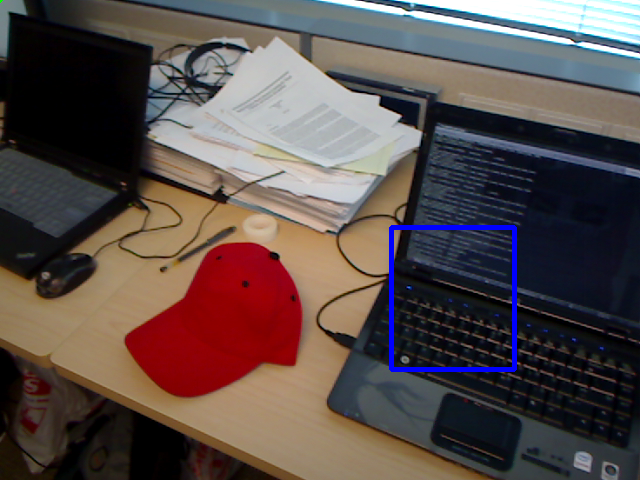
\includegraphics[width=\textwidth]{img/seguimiento_solo_frame/solo_frame-desk_1-coffee_mug_5-frame_34.png}
	\end{subfigure}

	\caption{Seguimiento frame a frame divergiendo. Aquí se estaba usando solo comparación de histogramas entre el frame anterior y el actual}
	\label{frame_only_tracking}
\end{figure}


\begin{figure}
	\centering
	\begin{subfigure}[b]{0.3\textwidth}
		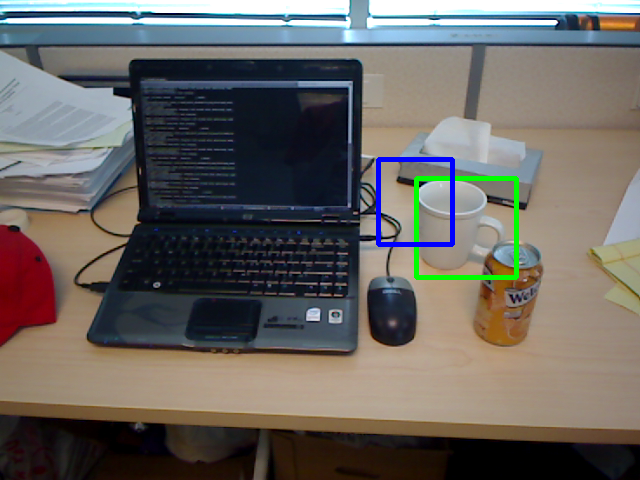
\includegraphics[width=\textwidth]{img/seguimiento_frame_template/frame_template-desk_1-coffee_mug_5-frame_26.png}
	\end{subfigure}
	\begin{subfigure}[b]{0.3\textwidth}
		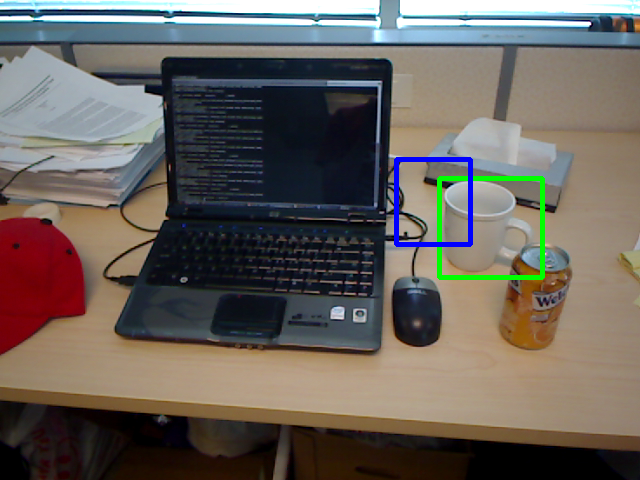
\includegraphics[width=\textwidth]{img/seguimiento_frame_template/frame_template-desk_1-coffee_mug_5-frame_27.png}
	\end{subfigure}
	\begin{subfigure}[b]{0.3\textwidth}
		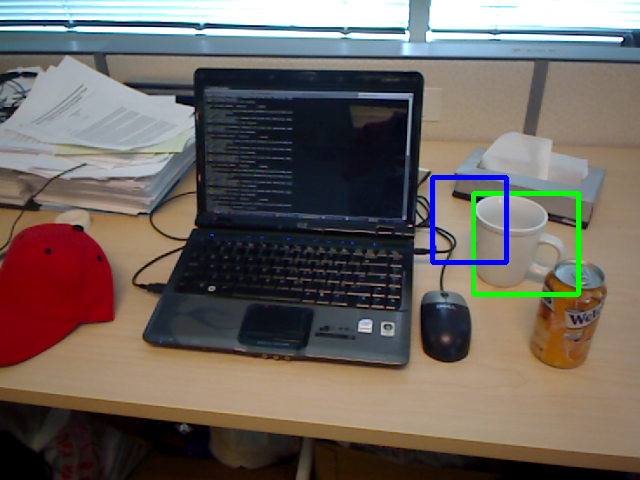
\includegraphics[width=\textwidth]{img/seguimiento_frame_template/frame_template-desk_1-coffee_mug_5-frame_28.png}
	\end{subfigure}


	\begin{subfigure}[b]{0.3\textwidth}
		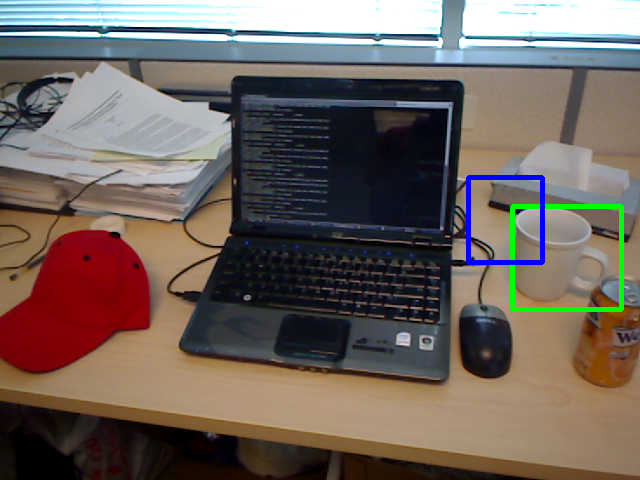
\includegraphics[width=\textwidth]{img/seguimiento_frame_template/frame_template-desk_1-coffee_mug_5-frame_29.png}
	\end{subfigure}
	\begin{subfigure}[b]{0.3\textwidth}
		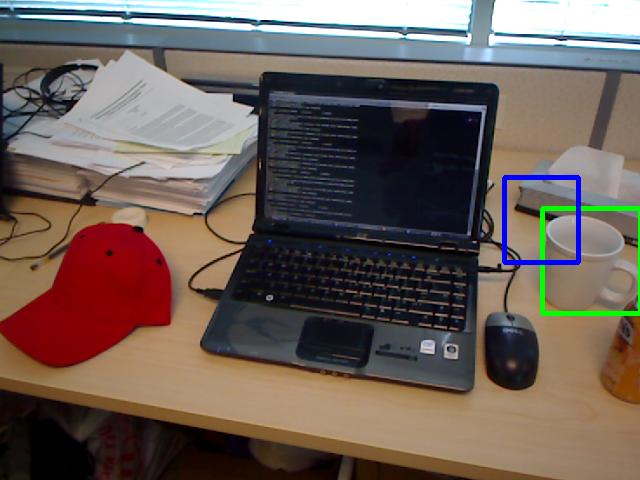
\includegraphics[width=\textwidth]{img/seguimiento_frame_template/frame_template-desk_1-coffee_mug_5-frame_30.png}
	\end{subfigure}
	\begin{subfigure}[b]{0.3\textwidth}
		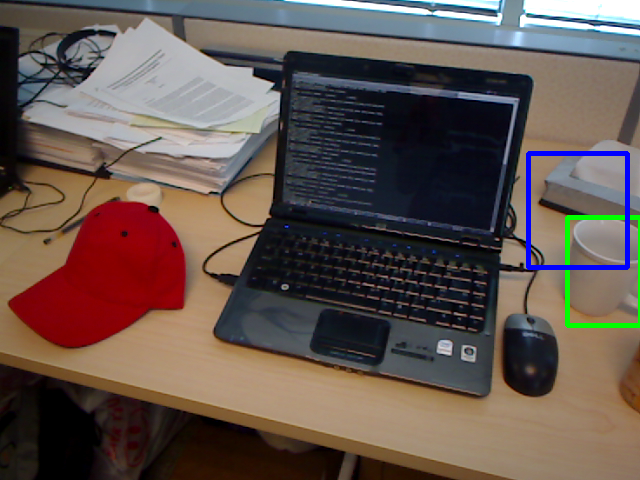
\includegraphics[width=\textwidth]{img/seguimiento_frame_template/frame_template-desk_1-coffee_mug_5-frame_31.png}
	\end{subfigure}

	\begin{subfigure}[b]{0.3\textwidth}
		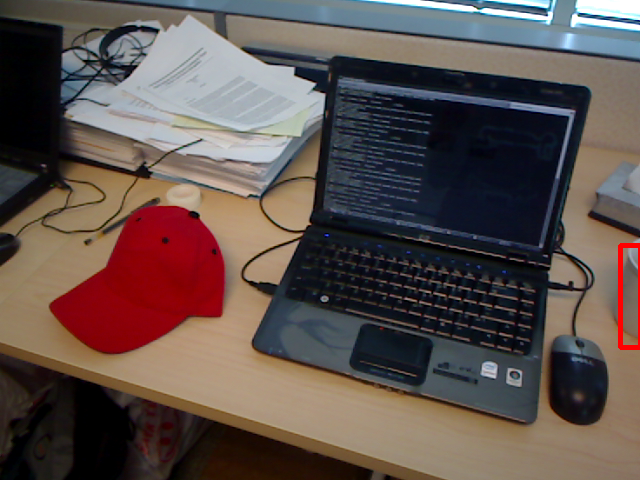
\includegraphics[width=\textwidth]{img/seguimiento_frame_template/frame_template-desk_1-coffee_mug_5-frame_32.png}
	\end{subfigure}
	\begin{subfigure}[b]{0.3\textwidth}
		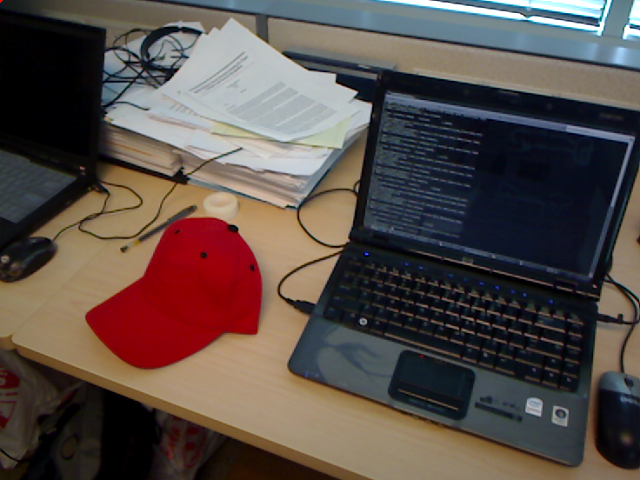
\includegraphics[width=\textwidth]{img/seguimiento_frame_template/frame_template-desk_1-coffee_mug_5-frame_33.png}
	\end{subfigure}
	\begin{subfigure}[b]{0.3\textwidth}
		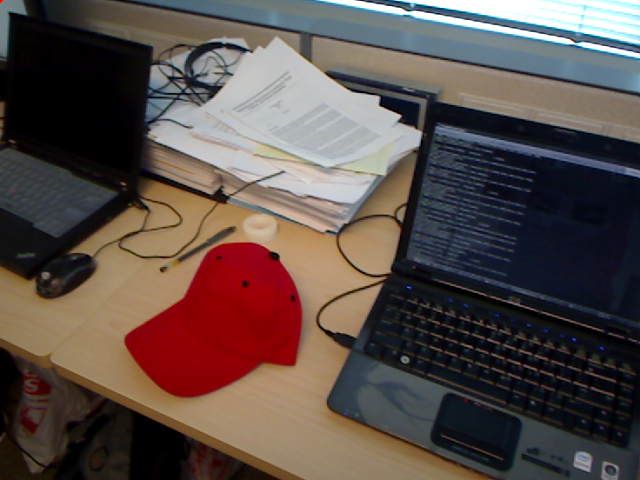
\includegraphics[width=\textwidth]{img/seguimiento_frame_template/frame_template-desk_1-coffee_mug_5-frame_34.png}
	\end{subfigure}

	\caption{Seguimiento frame a frame sin falsos positivos. Aquí se estaba usando las comparaciones de histogramas entre el frame anterior, el actual y el template del objeto}
	\label{frame_template_tracking}
\end{figure}

Una vez corridas estas dos sub-etapas dentro de la etapa de seguimiento, pueden ocurrir dos cosas. Una es si el algoritmo reportó haber encontrado al objeto. En este caso se almacenan los datos necesarios y se continúa utilizando el algoritmo de seguimiento en el frame siguiente. Si en cambio el algoritmo indica que el objeto no se encontró, se vuelve a la etapa de detección explicada previamente.



\section{Método propuesto en D}
\subsection{Alignment prerejective}\label{alignment_prerejective}
En esta sección explicaremos el método de estimación de pose proveniente del trabajo \cite{6630856}, el cual fue utilizado en gran parte de este trabajo.

El problema de determinar una transformación que permita alinear dos superficies ha generado muchas investigaciones en el campo de la visión en computación. Desde la manipulación de objetos en robótica hasta la reconstrucción de un modelo de un objeto o escena a partir de varias imágenes tomadas de distintos ángulos. En general estos métodos requieren una solución precisa para luego poder utilizar el resultado con otros problemas de procesamiento.

Hay muchos métodos conocidos para resolver este problema tanto en el dominio 2D como en el 3D y en general están basados en extracción de descriptores para eliminar falsas correspondencias entre las dos superficies o modelos. Es ampliamente conocido el hecho que los descriptores locales proveen una alta estabilidad dada su tolerancia al ruido y ocluciones. El objetivo de este trabajo era combinar inputs de ambos dominios de manera eficiente para resolver el problema de la estimación de pose.

En este trabajo realizan una serie de pasos bien definida hasta obtener una transformación como resultado final que indique la pose del objeto en la escena. En primer instancia, se obtienen puntos de interés utilizando un sistema ECV (\textit{Early Cognitive Vision}) cuya densidad está en un punto intermedio entre una imagen con puntos de interés escasos y descriptores de formas en 3D muy densos. Este sistema permite clasificar regiones de una imagen en tres categorías: región homogenea, región de borde y región con textura. En este trabajo se usan solo las últimas dos categorías ya que los pixeles en las regiones homogeneas resultan ser ambiguos para buscar correspondencias. Luego le agregan a cada descriptor información de sus vecinos, tanto de texturas como de formas, para aumentar la habilidad del método para distinguir falsas correspondencias. A esto lo llaman \textit{ECV context descriptors}.

Una vez recolectada esta información, utilizan \textit{RANSAC} para estimar una transformación que alinee el objeto con la escena. Formalmente lo que se busca es una transformación que minimice la suma de la diferencia de cuadrados entre los puntos del modelo y sus correspondencias en la escena. Para lograr esto se realizan los siguientes pasos:
\begin{enumerate}
	\item Tomar 3 o más puntos del objeto y sus correspondencias en la escena usando los descriptores de contexto ECV
	\item Estimar una transformacion usando esas correspondencias
	\item Aplicar la transformación al objeto
	\item Buscar \textit{inliers} usando búsqueda de vecinos cercanos entre el objeto transformado y la escena. Si el número de inliers es bajo, volver al primer paso
	\item Medir la diferencia de cuadrados usando los inliers y si es el menor valor encontrado guardar la transformación como resultado
\end{enumerate}

Esto puede repetirse durante las iteraciones que se pretendan o cuando la diferencia de cuadrados sea menor que un umbral dado. En este trabajo se agrega un paso novedoso a este esquema RANSAC enumerado previamente. Este paso asume una propiedad geométrica de objetos rígidos para descartar rápidamente malas correspondencias. En particular utilizan el hecho que las distancias se mantienen y hacen un chequeo de las diferencias entre las distancias de los bordes del polígono virtual formado por los puntos random tomados en el paso 1 tanto para el objeto como para la escena. Utilizando una medida de distancia entre estos valores y un umbral descartan rápidamente malas correspondencias. Si se asume que no se descartan potenciales poses que alinean bien los modelos, se obtiene la misma probabilidad de éxito de manera mucho más rápida.


\subsection{Iterative Closest Point (ICP)}\label{ICP}
En esta sección explicaremos el método de alineación de formas 3D, llamado \textit{Iterative Closest Point} (ICP) surgido en el trabajo \cite{besl1992method}. En este trabajo se intenta encontrar respuesta a uno de los principales problemas en visión en computación: dada cierta información 3D en un sistema de coordenadas de un sensor, que describe una forma que puede corresponder a un modelo y dado un modelo en una representación geométrica distinta, lograr estimar la rotación y traslación óptimas que permitan alinear las dos formas minimizando la distancia entre ambas, permitiendo así determinar la equivalencia de las mismas usando \textit{mean-square} como métrica de distancia.

El algoritmo presentado puede ser utilizado en múltiples tipos de representaciones de datos geométricos como conjunto de puntos, conjuntos de segmentos de líneas, curvas paramétricas, superficies paramétricas, etc. Además se puede utilizar cualquier otra representación siempre que se acompañe a la misma de un método para calcular el punto más cercano de esa forma a un punto digitalizado dado.

Además de necesitar una manera de calcular el punto más cercano, también es necesario un método para obtener la rotación y traslación de mínimos cuadrados. Para los objetivos de este trabajo era preferible usar un algoritmo basado en cuaterniones como el método de Horn, aunque si se necesitara un método para más de tres dimenciones, entonces el algoritmo más apropiado es utilizar SVD.

Finalmente, el algoritmo ICP requiere los siguientes pasos:
\begin{itemize}
	\item Se obtienen el conjunto de puntos a alinear y el modelo
	\item Se comienza la iteración fijando los vectores de alineación relativos al conjunto de puntos a alinear para obtener una representación de la transformación completa. Luego se repiten los siguientes pasos hasta que algún criterio de convergencia se satisfaga
	\begin{enumerate}
		\item Computar los puntos más cercanos
		\item Tomando esos puntos, computar la alineación
		\item Aplicar la transformación provista por la alineación
		\item Terminar la iteración cuando la diferencia del error cuadrático medio entre dos resultados sucesivos sea menor a un
	\end{enumerate}
 $\delta > 0$ dado
\end{itemize}

En este trabajo se demostró que este algoritmo converge monótonamente hacia un mínimo local con respecto a la distancia cuadrática media. Sin embargo, nada puede decirse sobre la convergencia hacia el mínimo global deseado.

El algoritmo no es útil si solo un subconjunto de los puntos se corresponde con el modelo o con un subconjunto del modelo. Lamentablemente esto sucede con la mayoría de los algoritmos de ``pareo'' de formas en 3D. Pero sigue resultando útil si todo el conjunto de puntos se corresponde con parte del modelo.

Entre las ventajas más importantes de este método está el hecho de que maneje los seis grados de libertad y que sea independiente de la forma de representación. Además no requiere de extracción de descriptores y puede ser fácilmente utilizado en conjunto con otros algoritmos. Por otro lado, una desventaja importante es que es susceptible a outliers. Esto tiene como extensión que el algoritmo no sirve para resolver el problema de segmentar objetos en una escena.



\subsection{Entrenamiento}
Para esta primera etapa existen varias posibilidades distintas que van desde utilizar una única nube de puntos hasta generar un modelo completo del objeto 3D alineando todas las nubes de puntos disponibles en la base. Durante las pruebas preeliminares realizadas los algoritmos respondieron bien utilizando una única nube de puntos como modelo del objeto. Este motivo sumado a que en este trabajo nuestro objetivo se enfocó en la etapa de tracking, nos llevaron a optar por utilizar una única nube de puntos del objeto como modelo. Además pensando en términos prácticos, es mucho más factible obtener rápidamente una única nube de puntos del objeto que deseamos seguir a obtener un modelo completo 3D del mismo.

En el caso de estudio de esta tesis, la nube de puntos del objeto a seguir se obtuvo de la base de datos explicada en el capítulo \ref{base_rgbd}. De manera similar al entrenamiento en RGB, se tomó como nube de puntos modelo del objeto a la nube proveniente de la imágen de rotación 0 de una de las escenas del objeto. Una vez almacenados estos datos, se continúa con la siguiente etapa que es la de detección.

\comentarioP{Relacionar con template matching}

\subsection{Detección}
Para esta segunda etapa se utilizó el método descripto en la sección \ref{alignment_prerejective} refinando el resultado con ICP. La elección del mismo se realizó luego de correr varias pruebas que corroboraran la factibilidad del mismo. En estas pruebas también se observó que si la región donde se buscaba el objeto era lo suficientemente pequeña la búsqueda era más robusta.\comentarioP{Mejor más chica?} Teniendo en cuenta esto se pensó en una variante para la detección que utilice el método elegido. Esta tiene como primer paso obtener el alto y el ancho del modelo del objeto a seguir y escalarlos. Considerando cada una de estas escalas, dividimos la escena en cuadrantes de ese tamaño y corrimos el método de detección en cada cuadrante. Con el fin de detectar el objeto cuando el mismo se extiende sobre dos o más regiones, la búsqueda se hizo utilizando un marco que recorre todos los cuadrantes y sus uniones, como puede observarse en la figura \ref{frames_solapados}. Notar que la división por cuadrantes solo se realizó en los ejes ``x'' e ``y'' y no en el eje ``z'' ya que las pruebas preeliminares dieron buenos resultados de esta manera. La detección se corre en cada uno de estos cuadrantes y puede suceder que:
\begin{itemize}
	\item No se encontró el objeto en ningún cuadrante: en este caso el algoritmo indica que el objeto no se encuentra en el frame
	\item Se encontró el objeto en un cuadrante
	\item Se encontró el objeto en varios cuadrantes: el algoritmo devuelve la mejor posición encontrada según un puntaje de buena alineación devuelto por el algoritmo \ap.
\end{itemize}

Si la detección es positiva, se refina la alineación corriendo ICP entre el modelo del objeto transformado por el método ``alignment prerejective'' y el cuadrante de la escena donde fue encontrado el mismo. Con el objetivo de comenzar el seguimiento en las mejores condiciones posibles, se intentan tomar los puntos del objeto buscado pertenecientes a la escena. Esto se realiza porque se asume que el objeto se va modificando cuadro a cuadro, ya sea por movimientos de la cámara o del objeto. Una de las formas para obtener los puntos del modelo del objeto en la escena es utilizando un \kdt\footnote{AGREGAR REFERENCIA A KDTREE}. \comentarioP{Explicar un poco que es un kdtree} Se arma un \kdt con los puntos provenientes del modelo alineado y se filtran uno a uno los puntos de la escena que se encuentren cerca de al menos un punto del modelo en un cierto radio de distancia. \comentarioM{Explicar el ajuste automatico del LEAF} Los puntos que surjan de esta búsqueda son los considerados como encontrados en la escena. Para que el algoritmo de búsqueda considere exitosa la detección, la cantidad de puntos filtrados de la escena debe ser mayor o igual al 50\% de los puntos del modelo original. Si todas estas etapas son superadas con éxito, se considera que el objeto fue encontrado y se pasa a la siguiente etapa de seguimiento. Si cualquiera de estos pasos fallara, se comienza nuevamente con la etapa de detección en el siguiente frame.


\subsection{Seguimiento (ex Método de seguimiento en profundidad)}
El método de seguimiento elegido para profundidad es ICP, explicado en la sección \ref{ICP}. En esta sección explicaremos cómo fue la selección de los parámetros para este método y los resultados obtenidos con los parámetros elegidos.

La implementación de ICP utilizada es la incluida en la librería ``Point Cloud Library'' \cite{Rusu_ICRA2011_PCL}. Esta implementación admite distintos parámetros para modificar el comportamiento del método. Los parámetros explorados son los siguientes:

\begin{enumerate}
	\item Distancia máxima de correspondencia: Si entre dos puntos existe una distancia mayor a este valor no se van a tener en cuenta para la búsqueda de correspondencias.
	\item Número de iteraciones máximo: Criterio de corte.
	\item Distancia mínima entre transformaciones: Criterio de corte. Si dos transformaciones consecutivas tienen una distancia menor a este valor, el algoritmo termina.
	\item Suma euclidea mínima: Criterio de corte. Es la diferencia euclidea mínima permitida entre dos pasos del algoritmo.
\end{enumerate}

Además, una vez que converge ICP la librería facilita el valor de la suma del cuadrado de las distancias de la nube de puntos inicial a la nube de puntos destino como medida de que tan buena es la alineación obtenida. Este valor se utiliza como umbral para decidir si la respuesta encontrada se considera correcta o no, por lo que también se explora como el resto de los parámetros. A modo de refinar aún más el resultado, una vez hallada una buena alineación se procede a tomar los puntos de la escena que suponen ser los del objeto que se estaba buscando. La explicación de cómo se realiza este filtrado se puede ver en \comentarioM{EXPLICACION USO DE KDTREE. EXPLICAR EL AUTOAJUSTE DEL LEAF PARA KDTREE}. Una vez filtrados los puntos de la escena se compara esta cantidad de puntos con la cantidad de puntos que tiene el modelo del objeto. Si los puntos de la escena superan un porcentaje de puntos del modelo se considera que el objeto fue encontrado. Este porcentaje también es uno de los parámetros explorados.


\section{Método propuesto en RGB-D}\label{metodo_rgbd}

\subsection{Entrenamiento}

\subsection{Detección}

\subsection{Seguimiento}\label{tracking_rgbd}










\chapter{Base de datos RGB-D}\label{base_rgbd}
Durante el desarrollo de este trabajo se utilizaron secuencias con información de \textit{ground truth} de imágenes RGB-D con el objetivo de aplicar los métodos estudiados y tener una referencia para hacer comparaciones y sacar conclusiones sobre su eficacia. Las escenas fueron tomados del trabajo de Kevin Lai et al. \cite{lai2011large} en donde se creó una base de objetos y escenas. Esta base cuenta con 20 escenas y cada una de ellas contiene entre 100 y 200 frames RGB-D. El ground truth de esta base provee información frame a frame de qué objetos aparecen y cuál es su ubicación en el plano XY.

{\huge Figura con ejemplos de las escenas, por ejemplo: 2 filas con varias columnas cada una en donde haya frames RGB arriba y sus equivalentes en depth abajo}

Por otra parte, la base provee imágenes RGB-D de los objetos presentes en las escenas capturadas aisladamente con el objetivo de obtener su representación 3D.\comentarioP{Comentar como fueron adquiridas la resolución, longitud y ¿?} Cada una de estas imágenes es acompañada además por una máscara que segmenta al objeto buscado y la información de profundidad (nube de puntos) del objeto. Para tomar estas imágenes los objetos fueron ubicados en una base circular giratoria y, manteniendo la cámara en una posición fija, se tomaron muestras con cierta regularidad cubriendo toda la circunferencia de cada objeto. Esto se hizo además desde distintas alturas permitiendo apreciar la profundidad del objeto y así obtener una mejor descripción del mismo.

Los objetos elegidos para esta base se organizaron de una manera jerárquica tomada de las relaciones hiperónimo/hipónimo de WordNet. Cada objeto pertenece a una clase de objetos y hay varias instancias por cada clase. Por ejemplo, en la categoría ``taza'' existen varias instancias diferentes, que se corresponden simplemente a distintas tazas ya sea por forma o por color.

Existen distintas escenas que contienen a los objetos mencionados y en cada escena se combinan distintas clases de objetos y distintas instancias de la misma clase. De esta manera la base otorga la posibilidad de verificar algoritmos capaces de identificar instancias de objetos particulares o familias de objetos según la clasificación antes mencionada. En esta tesis usaremos .....
